\documentclass[a4paper]{article}

\usepackage{hyperref}
\usepackage{amsmath}
\usepackage{algorithmic}
\usepackage{algorithm}
\usepackage{graphicx}

\author{Paul van der Walt\footnote{\url{paul@@denknerd.org}}\\ \url{http://github.com/toothbrush/bsp-cg}}
\date{\today}
\title{A Parallel CG Algorithm\footnote{This work is inspired by Exercise 4.6 of PSC\cite{bisseling2004parallel}}}


\begin{document}

\maketitle

\begin{abstract}
    This is abstract
\end{abstract}

\newcommand{\ve}[1]{\ensuremath{\vec{#1}}}
\newcommand{\mat}[1]{\ensuremath{\boldsymbol{#1}}}
\newcommand{\plotsize}{0.7\textwidth}
\newcommand{\legendplotsize}{1.3\textwidth}
\section{Introduction}

A well-known problem in problem in first-year courses on linear algebra is the question that
given some matrix \mat{A} and some vector \ve{b}, give \ve{x} such that the equation $\mat A \ve x = \ve b$ holds. A human would probably do Gaussian elimination, but
in scientific computing, a very widely used algorithm that comes to mind is the conjugate gradient method, which can iteratively compute the solution of a linear system of equations whose matrix is \emph{symmetric} and \emph{positive definite}.
As is well-known, a matrix is symmetric when $\mat A = \mat A^T$ holds, and positive definite is defined as the property that $\ve x^T \mat A \ve x > 0$, for all $\ve x \neq \ve 0$.

The conjugate gradient algorithm is given in Algorithm \ref{alg:seq-cg}, and is due to Hestenes and Stiefel \cite{hestenes1952methods}. It has been proven that the algorithm converges \cite{golub1996matrix}.

\begin{algorithm}
    \caption{Sequential conjugate gradient algorithm.}
\label{alg:seq-cg}
\begin{algorithmic}
    \REQUIRE ~\\
             $\mat A$ symmetric, positive definite, $n\times n$ matrix,\\
             $\ve  b$ vector of length $n$
    \ENSURE  $\mat A \ve x = \ve b$\\~\\
    \STATE $\ve x \leftarrow \ve{x_0}$ \COMMENT{initial guess}
    \STATE $k \leftarrow 0$ \COMMENT{iteration number}
    \STATE $\ve r \leftarrow \ve b - \mat A \ve x$
    \STATE $\rho \leftarrow ||\ve r||^2$
    \WHILE{$\sqrt{\rho} > \epsilon ||\ve b|| \wedge k < k_{max}$}
        \IF{$k=0$}
            \STATE $\ve p \leftarrow \ve r$
        \ELSE
            \STATE $\beta \leftarrow \rho/\rho_{old}$
            \STATE $\ve p \leftarrow \ve r + \beta \ve p$
        \ENDIF
        \STATE $\vec w \leftarrow \mat A \ve p$
        \STATE $\gamma \leftarrow \ve p . \ve w$
        \STATE $\alpha \leftarrow \rho/\gamma$
        \STATE $\ve x  \leftarrow \ve x + \alpha \ve p$
        \STATE $\ve r  \leftarrow \ve r - \alpha \ve w$
        \STATE $\rho_{old} \leftarrow \rho$
        \STATE $\rho   \leftarrow || \ve r || ^2$
        \STATE $k \leftarrow k+1$
    \ENDWHILE
\end{algorithmic}
\end{algorithm}


\section{The sequential algorithm}

To get a feel for the algorithm the first step was to implement a sequential version. The source code 

\section{The parallel algorithm}

\subsection{Complexity}

\subsection{Data distribution}

\section{Matrix generation}\label{sec:matrix-generation}

% talk a bit about genmat.c

\section{Experimental results}

A number of experiments were done to explore what the effect of varying $p$,
$N$, nonzero density or processor distribution would be. Specifically, series
of matrices was generated to measure the running time with varying $p$ (section
\ref{sec:time-run}), running time with varying load imbalance (section
\ref{sec:imbalance-run}), and running time with varying $N$ (section
\ref{sec:nz-run}).

In each case, the matrices were generated, and the vector to solve for
was generated on-the-fly by the \texttt{cg} program, with real values
in the range $[0,1)$. The random seed was hard-coded into the program,
    so subsequent runs would produce the same outcome.

The running times mentioned are only counting the time taken by the main CG loop
in the program; initial loading of distributions from files and the distribution of
nonzero values to their destination processors is considered startup time, and is therefore
ignored. This also makes comparison of results more compatible.

\subsection{Varying $p$}\label{sec:time-run}

In this experiment, a number of matrices with varying $N$ and nonzero density (referred to as $\delta$) were generated and
subsequently distributed using Mondriaan\footnote{The settings used for Mondriaan
were the defaults, using a load imbalance of 0.3.} for 1, 2, 4 and 8 processors. Table \ref{tbl:time-run} lists the actual matrix configurations used. The runtimes for each matrix are displayed in Figure \ref{fig:time-run}.

\begin{table}
    \centering
    % foreach matrix write N, density, final nz
    \begin{tabular}{l|l|l|l}
        $N$ & $\delta_{aim}$ & $nz$ & $\delta$ \\ \hline
1000  &  0.001   &   2000   &   0.002\\
2000  &  0.001   &   5966   &   0.00149\\
1000  &  0.005   &   6032   &   0.006\\
1000  &  0.01   &   11044   &   0.011\\
2000  &  0.005  &   22030   &   0.0055\\
5000  &  0.001   &   29914   &   0.00120\\
2000  &  0.01   &   42228   &   0.0106\\
10000  & 0.001    &   110152   &   0.0011\\
5000  &  0.005   &   130212   &   0.0052\\
5000  &  0.01  &   256504   &   0.01026\\
20000  & 0.001    &   420412   &   0.00105\\
10000  & 0.005   &   511034   &   0.00511\\
10000  & 0.01   &   1015308   &   0.0102\\
20000  & 0.005    &   2024134   &   0.0051\\
20000  & 0.01    &   4041652   &   0.0101\\
10000  & 0.1    &   10536950   &   0.105\\
5000  &  0.5   &   16668124   &   0.6668\\
    \end{tabular}
    \caption{The matrices used for measuring the speedup of using more processors to solve a fixed problem. $N$ is the size of the sparse matrix \mat A (number of rows and columns), $\delta_{aim}$ is the sparsity the matrix generator was aiming for, $nz$ the final number of nonzeroes, and $\delta$ the actual density. In most cases, $\delta$ has been rounded.}
    \label{tab:time-run}
\end{table}

The first thing one notices when looking at Table \ref{tab:time-run} is that the actual densities of
the generated matrices is not precisely equal to the density $\delta_{aim}$ provided to the program
\texttt{genmat} which generated the test matrices. The reason for this is the way the matrices are
randomly generated, and is discussed in more detail in Section \ref{sec:matrix-generation}.

When looking globally at Figure \ref{fig:time-run} we see behaviour that we would expect: when
using more processors to solve a problem, the run time is less. More subtle is the detail that the
speedup is much more dramatic for larger (in terms of the number of nonzero entries) matrices than for smaller
ones. This can be explained by the fact that if a given processor doesn't have much work to do, the
amount of communication needed will be relatively great, whereas when a very large problem is distributed among
many processors, each processor still has enough work to be kept busy.

We also see that in general, the larger the matrix, the longer the run time, regardless of how many processors
are used. There are one or two small exceptions, but in general, a larger matrix will take strictly more computing
time. The exceptions to this observation are explained by the fact that on Huygens we make use of
shared nodes, so a given node might have been busier when solving a smaller matrix, and that by chance when
solving a larger matrix, we had the whole node to ourselves. The differences are however insignificant and
within acceptable tolerance to be explained this way.

\begin{figure}[h]
    \begin{center}
        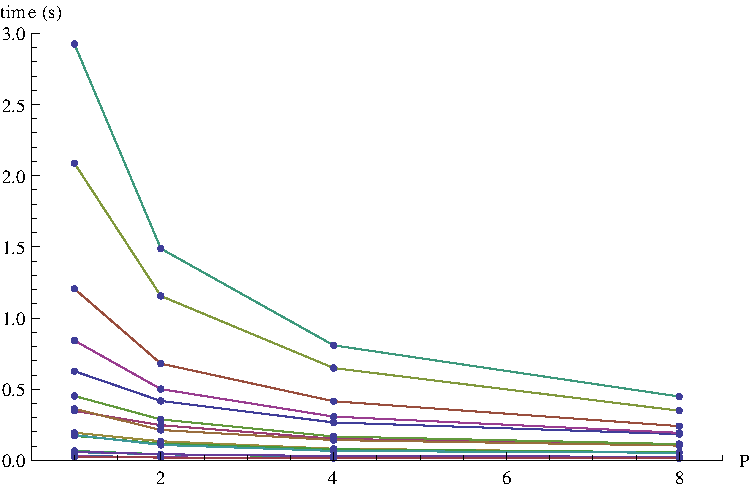
\includegraphics[width=\legendplotsize]{img/time-run.pdf}
    \end{center}
    \caption{Varying $P$ while keeping other factors constant.}
    \label{fig:time-run}
\end{figure}


Next, one might wonder how great the advantage actually is of distributing a given matrix over $P$ processors.
This is explored in Figure \ref{fig:speedup}. Here, we have taken the curves from Figure \ref{fig:time-run} and
taken the inverse ($1/x$) of each value, after which the values were all scaled by the value for the case
when $P=1$. This way we can see how many times faster a given run was when run on $P>1$ cores compared to
when just one (sequential case) was used.




\begin{figure}[h]
    \begin{center}
        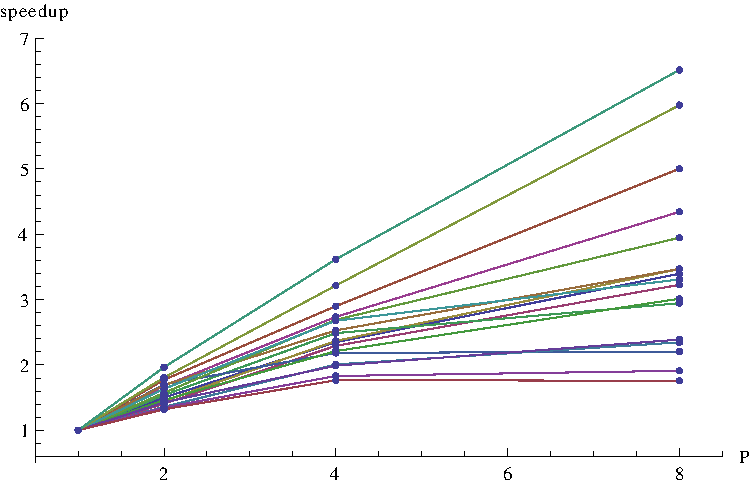
\includegraphics[width=\legendplotsize]{img/speedup.pdf}
    \end{center}
    \caption{The speedup achieved by increasing $P$ with various matrices.}
    \label{fig:speedup}
\end{figure}


Here we see an interesting phenomenon. For the larger matrices, the speedup is rather dramatic
(at most 10\% less than $P$), whereas the smaller matrices have little or no speedup after $P=2$. The
reason for this is what was touched upon earlier: when a problem is too small to sensibly distribute over
many processors, the communication becomes relatively expensive compared to the computation time. Just as we
wouldn't hire 8 people to help us eat a sandwich, a banquet can be devoured a lot more efficiently by many
people than if we were to try and finish it on our own.

In other words, for a given matrix size, there is an optimal number of processors to use
to solve the problem. If we use more, we're slowing the process down again.


\subsection{Varying $N$}\label{sec:nz-run}

Something which was purposely left a little vague in the previous section is the
influence that density has on the performance of our solver. One might wonder if the number of nonzeroes,
the density of the matrix, or both has an impact, and if so, how much.

To this end, a few matrices of varying size were generated using two target densities, $\delta=0.1$ and $\delta=0.2$, with
the matrix dimensions chosen such that the number of nonzeroes generated would be in the same order of magnitude each
time. The matrices used are summarised in Table \ref{tab:nz-mats}. They were all partitioned
using Mondriaan for $P=2$ and load imbalance 0.1.

The results are plotted in Figure \ref{fig:density-run}.

\begin{table}
    \centering
    \begin{tabular}{l|l|l|l}
        $N$ & $\delta_{aim}$ & $nz$ & $\delta$ \\ \hline
1000  & 0.1   &   106342   &   0.106\\
1000  & 0.2   &   223034   &   0.223\\
2000  & 0.1   &   423252   &   0.1058\\
2000  & 0.2   &   889372   &   0.222\\
3000  & 0.1   &   950022   &   0.1056\\
4000  & 0.1   &   1689062   &   0.1056\\
3000  & 0.2   &   2001058   &   0.222\\
4000  & 0.2   &   3555962   &   0.222\\
6000  & 0.1   &   3797120   &   0.1055\\
8000  & 0.1   &   6745868   &   0.1054\\
5657  & 0.2   &   7110505   &   0.222\\
    \end{tabular}
    \caption{A number of matrices generated with different target densities $\delta_{aim}$, but
with dimensions $N$ chosen such that the number of nonzeroes, $nz$, would be comparable.}
    \label{tab:nz-mats}
\end{table}


\begin{figure}[h]
    \begin{center}
        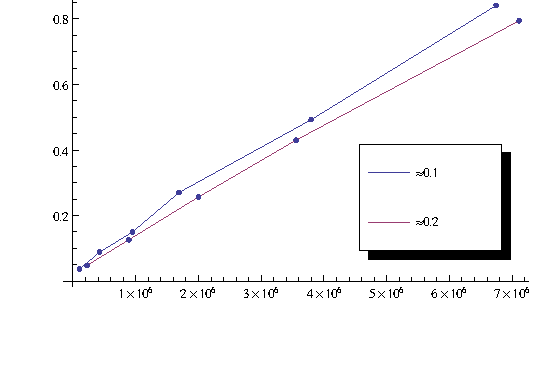
\includegraphics[width=\plotsize]{img/density-run.pdf}
    \end{center}
    \caption{Varying $N$ while maintaining two constant densities. $P=2$}
    \label{fig:density-run}
\end{figure}

The first observation that can be made is that it is evident that the absolute number of
nonzero entries for a given matrix has more influence on the run time than the density
(or, by the same token, the dimension $N$). We do, however, notice a fairly constant
slowdown of the sparser matrices when compared to the denser matrices. This can be explained
by thinking about how matrices are partitioned for many processors. Given a certain matrix with
a certain nonzero pattern, if we double the size $N^2$ but halve the density (to achieve a similar
number of nonzeros), what might happen is that instead of having a single vector on some processor
with some nonzeros, it is now split into to, which potentially causes communication. This makes the
matrix more difficult to partition, which is most likely where the speed penalty comes from. In this
light, given a number of nonzeros $nz$, it is preferable to have a matrix with smaller $N$ and higher
density, as far as solving speed goes. Having said all this though, the time difference is
still very minimal.

\subsection{Varying load imbalance}\label{sec:imbalance-run}

Since for each set of matrices that has been generated, we've used Mondriaan to
distribute them to minimise communication and load imbalance, it's interesting to
measure what the impact is of varying the only parameter we've given Mondriaan, namely
the maximum load imbalance. For this experiment, a single test matrix ($N=6000$, $\delta_{aim}=0.1$) was generated and distributed
over 8 processors, but each time with a different maximal load imbalance. The
values used for load imbalance were $\varepsilon = \left\{  0.1, 0.3, 0.6, 0.8\right\}$. The results
are plotted in Figure \ref{fig:imbalance}.

\begin{figure}[h]
    \begin{center}
        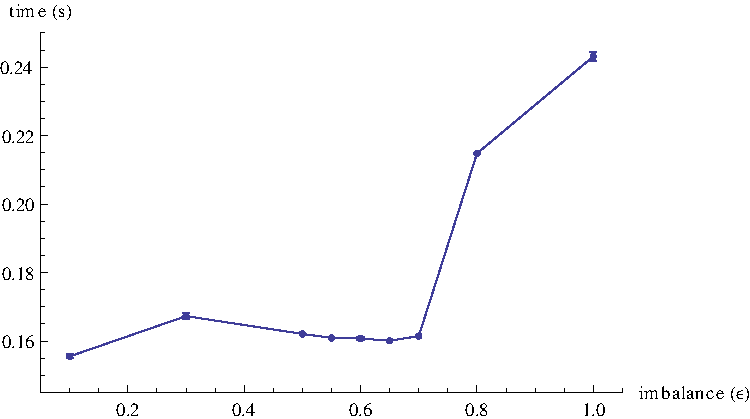
\includegraphics[width=\plotsize]{img/imbalance.pdf}
    \end{center}
    \caption{The load imbalance's effect on run time. $N=6000$, $P=8$, $\delta_{aim}=0.1$}
    \label{fig:imbalance}
\end{figure}

%TODO

mention final nz and density of matrix
mention error bars

\section{Conclusion}


\appendix
\clearpage
\section{Bug fixed in BSPedupack}

After some experiments with the latest versions of BPSonMPI, OpenMPI and
BSPedupack, it became clear that there was a bug causing the parallel matrix-vector
multiplication function
\texttt{bspmv} to always return a zero-array (i.e. instead of the result vector
\texttt{u} containing the answer to the multiplication of some \texttt{A} and
\texttt{v}, it only contained zeroes), when run on a local Linux machine (the
problem didn't appear using the IBM compiler on Huygens).

The problem turned out to be that the function \texttt{bspmv} used
\texttt{bsp\_set\_tag\_size} with a second argument of type \texttt{int},
instead of \texttt{size\_t}, which BSPonMPI requires. When this had been
changed (no other changes to the code were necessary), the examples compiled
without warnings once again, and ran fine, producing the expected answers.

The surprising thing was that previously BSPedupack had functioned without
problems on my systems (Linux x86-64 and OS X), and it still worked on Huygens,
which probably means they have an older library somewhere, or that their
compiler (as opposed to my GNU CC compiler) is less strict in casting \texttt{size\_t} to \texttt{int} and vice versa.

The difference between \texttt{size\_t} and \texttt{int}, is that the former is
independent of the underlying architecture, while an \texttt{int} has a width
which depends on the processor's instruction size. Evidently the IBM compiler
is lenient and casts \texttt{int} to the struct \texttt{size\_t} without
problems, but the GNU CC compiler sets the value of the \texttt{size\_t} to 0.

For completeness a diff has been included, which shows exactly what needed patching.

% git diff e2fa992c414d3811e99fc3e361ebfa921178de86 46707e6e774b2b3436a0b3361326fe99df5c7022

\begin{verbatim}
diff --git a/src/libs/bspmv.c b/src/libs/bspmv.c
index 5dabc65..a05a2f1 100644
--- a/src/libs/bspmv.c
+++ b/src/libs/bspmv.c
@@ -49,9 +49,15 @@ void bspmv(int p, int s, int n, int nz, int nrows, int ncols,
        u[k] is the k'th local component of u, 0 <= k < nu.
     */
 
-    int i, j, k, tagsz, status, nsums, nbytes, *pinc;
+    int i, j, k, status, nsums, *pinc;
     double sum, *psum, *pa, *vloc, *pvloc, *pvloc_end;
 
+#ifdef __GNUC__
+    size_t tagsz, nbytes;
+#else
+    int tagsz, nbytes;
+#endif
+
     /****** Superstep 0. Initialize and register ******/
     for(i=0; i<nu; i++)
         u[i]= 0.0;
diff --git a/src/libs/vecio.c b/src/libs/vecio.c
index 052138d..958e64d 100644
--- a/src/libs/vecio.c
+++ b/src/libs/vecio.c
@@ -44,7 +44,12 @@ void bspinput2triple(char*filename, int p, int s, int *pnA, int *pnz,
        ja[k] is the global column index.
     */
 
-    int pA, mA, nA, nzA, nz, q, nzq, k, tagsz, status, *Pstart, *ia, *ja;
+    int pA, mA, nA, nzA, nz, q, nzq, k, status, *Pstart, *ia, *ja;
+#ifdef __GNUC__
+    size_t tagsz;
+#else
+    int tagsz;
+#endif
     double value, *a;
     indexpair t;
     FILE *fp;
\end{verbatim}
\clearpage

\section{Experimental data}

If one should want to duplicate the results found in this report, all that needs to be done
is to make a clone of the GitHub repository containing this project, which can be found at
\url{http://github.com/toothbrush/bsp-cg}. If one would like to try running the programs on the exact matrices
used to generate the results presented here, an archive containing all the matrices with their
different partitionings ($P=1,2,4,8, \ldots$) is provided (warning: large
download) at \url{http://denknerd.org/} %TODO provide matrices online

The archive contains a number of folders, which correspond to the various experimental runs
presented in this report. Each folder contains one or more \texttt{*.emm} files, which are the original
matrices as generated by \texttt{genmat}, and finally, the files \texttt{*.emm-$\left\{\texttt{P,u,v}\right\}n$} are
the output after having run Mondriaan on the corresponding \texttt{emm} file to partition the matrix for $n$ processors.

A partitioned matrix can be run using the compiled \texttt{cg} tool, which implements the parallel CG solver. On
a usual desktop machine with OpenMPI, the invocation would be (assuming the current working directory is in
the root of the code repository):

\begin{verbatim}
$ make
$ mpirun -np N ./bin/cg mats/something.emm-{P,u,v}N
\end{verbatim}

Where $N$ stands for the number of processors desired, so an example of a concrete invocation could be:
\begin{verbatim}
$ mpirun -np 2 ./bin/cg mats-timing-experiment/linsys-5000-0.010000.emm-{P,u,v}2
\end{verbatim}

After loading the matrix and vector distributions, the solver is automatically
run, and finally some results are presented. When not in debug-mode (selected by compiling
with the \texttt{-DDEBUG} flag), the actual solution isn't presented, only the loading and
initialisation time, the solving time, and some other statistics like the number of iterations
and final error achieved.

The matrices for the first experiment, mentioned in Section \ref{sec:time-run}, are also provided
in Mathematica format, in the files \texttt{mat-check-*.nb}. These files are also generated by \texttt{genmat} and
were initially useful for making sure the generated matrices had the desired properties of being
symmetric and positive definite. Although now redundant, these files are also provided for interest's sake.

\clearpage
\section{Homebrew}

As an aside to this project, it seems beneficial to mention the existence of a
tool called Homebrew\footnote{\url{http://mxcl.github.com/homebrew/}}, which is
a package manager for OS X. It is similar to package management systems found
on many Linux distributions, such as apt on Debian or yum on Red Hat. Since the
author of this report is lazy and didn't feel like installing OpenMPI and
BSPonMPI from source each time, an installation script for BSPonMPI was added,
so that users of Homebrew (which is highly recommended above Fink or MacPorts,
for example) can suffice with running something like the following to get an
environment which enables the compilation and execution of this project.

\begin{verbatim}
$ brew update
$ brew install bsponmpi
\end{verbatim}

If it is not already installed, OpenMPI will be installed as a dependency of BSPonMPI.

\section{Code listings}
% here we need
% the bspcg.c


\bibliographystyle{plain}
\bibliography{cg}
\end{document}
